%% start of file `template.tex'.
%% Copyright 2006-2013 Xavier Danaux (xdanaux@gmail.com).
%
% This work may be distributed and/or modified under the
% conditions of the LaTeX Project Public License version 1.3c,
% available at http://www.latex-project.org/lppl/.

\documentclass[11pt,a4paper,sans]{moderncv}        % possible options include font size ('10pt', '11pt' and '12pt'), paper size ('a4paper', 'letterpaper', 'a5paper', 'legalpaper', 'executivepaper' and 'landscape') and font family ('sans' and 'roman')

% modern themes
\moderncvstyle{banking}                            % style options are 'casual' (default), 'classic', 'oldstyle' and 'banking'
\moderncvcolor{orange}                                % color options 'blue' (default), 'orange', 'green', 'red', 'purple', 'grey' and 'black'
%\renewcommand{\familydefault}{\sfdefault}         % to set the default font; use '\sfdefault' for the default sans serif font, '\rmdefault' for the default roman one, or any tex font name
%\nopagenumbers{}                                  % uncomment to suppress automatic page numbering for CVs longer than one page

% character encoding
\usepackage[utf8]{inputenc}                       % if you are not using xelatex ou lualatex, replace by the encoding you are using
%\usepackage{CJKutf8}                              % if you need to use CJK to typeset your resume in Chinese, Japanese or Korean

% adjust the page margins
\usepackage[scale=0.75]{geometry}
%\setlength{\hintscolumnwidth}{3cm}                % if you want to change the width of the column with the dates
%\setlength{\makecvtitlenamewidth}{10cm}           % for the 'classic' style, if you want to force the width allocated to your name and avoid line breaks. be careful though, the length is normally calculated to avoid any overlap with your personal info; use this at your own typographical risks...

\usepackage{import}
\usepackage{color}
\usepackage{geometry}
% personal data
\name{Pierre}{Avital}
\title{}                               % optional, remove / comment the line if not wanted
\address{1bis rue Jean Mermoz}{78500}{Sartrouville}% optional, remove / comment the line if not wanted; the "postcode city" and and "country" arguments can be omitted or provided empty
\phone[mobile]{+33630824860}                   % optional, remove / comment the line if not wanted
%\phone[fixed]{01234 123456}                    % optional, remove / comment the line if not wanted
%\phone[fax]{+3~(456)~789~012}                      % optional, remove / comment the line if not wanted
\email{pierre.avital@gmail.com}                               % optional, remove / comment the line if not wanted
%\homepage{www.myname.webs.com}                         % optional, remove / comment the line if not wanted
\extrainfo{Permis B + Véhicule}                 % optional, remove / comment the line if not wanted
\photo[64pt][0.4pt]{DSC_0296.JPG}                       % optional, remove / comment the line if not wanted; '64pt' is the height the picture must be resized to, 0.4pt is the thickness of the frame around it (put it to 0pt for no frame) and 'picture' is the name of the picture file
%\quote{}                              % optional, remove / comment the line if not wanted

% to show numerical labels in the bibliography (default is to show no labels); only useful if you make citations in your resume
%\makeatletter
%\renewcommand*{\bibliographyitemlabel}{\@biblabel{\arabic{enumiv}}}
%\makeatother
%\renewcommand*{\bibliographyitemlabel}{[\arabic{enumiv}]}% CONSIDER REPLACING THE ABOVE BY THIS

% bibliography with mutiple entries
%\usepackage{multibib}
%\newcites{book,misc}{{Books},{Others}}
%----------------------------------------------------------------------------------
%            content
%----------------------------------------------------------------------------------
\geometry{bottom=1cm,top=2.5cm}
\begin{document}
%\begin{CJK*}{UTF8}{gbsn}                          % to typeset your resume in Chinese using CJK
%-----       resume       ---------------------------------------------------------
\begin{picture}(0,0)
\put(385,0){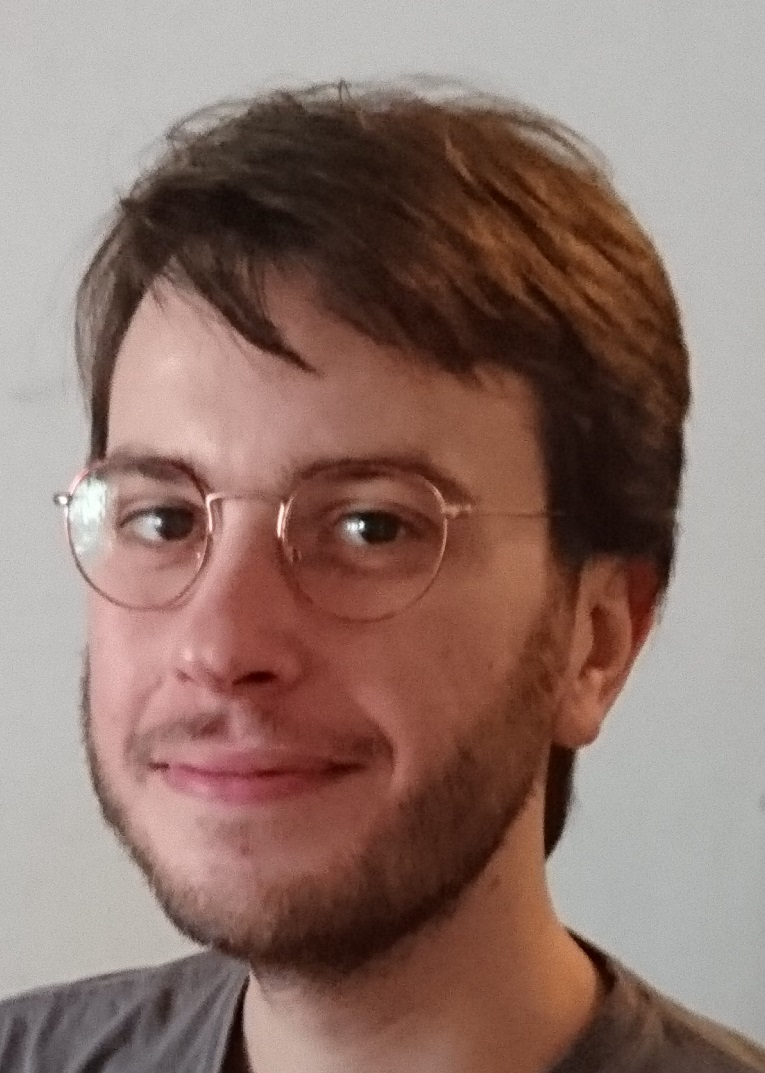
\includegraphics[scale=0.08]{DSC_0296.JPG}}
\end{picture}
\put(140,-11){\color{gray}Double nationalité : Français - Suisse}
\makecvtitle

\small{Double diplômé \textbf{Ingénieur Technologies Mobiles et Systèmes Embarqués} / \textbf{Master Sécurité des Systèmes d'Information} en Septembre de cette année, je suis à la recherche d'un emploi à partir d'Octobre. Je souhaiterais particulièrement mettre mes compétences variées au service de la recherche.}

\section{Expérience}

\vspace{6pt}

\begin{itemize}

\item{\cventry{Novembre 2017 - Mars 2018}{Ingénieur recherche et développement}{Valeo}{Créteil}{}{\vspace{3pt}TODO:DESCRIPTION DU POSTE}}

\vspace{6pt}

\item{\cventry{Février 2017 -- Aout 2017}{Stage de fin d'études : sécurité des véhicules connectés}{Pôle Judiciaire de la Gendarmerie Nationale}{Pontoise}{}{\vspace{3pt}Partant de l'étude de la sécurité d'applications Android, j'ai développé un plugin d'intégration pour Atom nommé SmalIntegrate basé sur des outils open-source transformant cet éditeur de texte en IDE spécialisé pour le reverse d'applications Android.\\J'ai également développé une preuve de concept d'écoute de la bande ISM 2.4GHz à l'aide d'une SDR et de recherche de signaux Bluetooth sans information préalable dans le signal obtenu.\\\textit{Technologies : Atom, ADB, JDB, GNU Radio, Quartus Prime, FPGA, Gateware, Firmware, DSP, Sans-fil\\Langages : Assembleur (Dalvik), JavaScript, Bash, Python, VHDL}}}

\vspace{6pt}

\item{\cventry{Septembre 2015 -- Février 2016}{Stage : développement d'innovation et conseil scientifique}{Castrol innoVentures}{Reading, UK}{}{\vspace{3pt}InnoVentures est l'incubateur d'innovation de Castrol (BP). Au sein d'une équipe issue de diverses cultures et formations, j'y ai agi en tant que consultant scientifique et ai participé au développement de divers projets en suivant les méthodologies issues du monde des start-ups.}}

\end{itemize}

\section{Parcours scolaire}

\vspace{5pt}

\subsection{Parcours universitaire}

\vspace{5pt}

\begin{itemize}

\item{\cventry{2011--2017}{Ingénieur Technologies Mobiles Systèmes Embarqués / Master Sécurité des SI}{Université de Technologie de Troyes}{Troyes}{}{Obtenant lors du Tronc Commun une solide formation en Mathématiques, Physique, Électronique et Chimie, je me suis distingué au cours de mon cursus ingénieur par mon intérêt particulier pour le bas niveau et le traitement de signal. J'ai complété ma formation d'un master SSI où j'ai excellé en cryptographie.}}

\end{itemize}

\vspace{2pt}

\subsection{Projets principaux}

\vspace{5pt}

\begin{itemize}

\item{TX - Vision embarquée sur carte Zynq}

\vspace{3pt}

\small{Le but de ce projet était l'étude des capacités de la carte Zynq, hybride contenant un processeur ARM ainsi qu'un circuit logique programmable (FPGA), particulièrement dans le domaine de l'accélération matérielle pour le traitement d'images.}

\vspace{6pt}

\item{FSG002 - Fox Music Analysis Library}

\vspace{3pt}

\small{Codée en C\#, cette bibliothèque d'analyse musicale avait pour but originel l'analyse en temps réel de musiques pour permettre l'intégration de celles-ci à des mécaniques de jeu. Plus tard, son but a évolué en la création d'un support de retranscription automatique de musiques en partitions ou fichiers MIDI.}

\vspace{6pt}

\item{Danish!}

\vspace{3pt}

\small{Une implémentation en Java du jeu de bataille norvégienne. Suivant le patron de conception MVC, et ayant eu un cycle de développement en cascade.}

\end{itemize}
\newpage
\section{Compétences}

\vspace{6pt}

\begin{itemize}

\item \textbf{Langues} 
\begin{itemize}
\item Français : Langue natale
\item Anglais : Courant, avec une connaissance approfondie du langage technique et scientifique. BULATS C1 (2012), Erasmus C2 (2016), 9 mois cumulés en pays anglo-saxons, dont 6 en stage à Reading, UK.
\item Allemand : Niveau scolaire. B1/B2. 1 mois cumulé en pays germanophones.
\item Japonais : Capacité à converser. 3 semaines passées en voyage personnel en 2014.
\end{itemize}

\vspace{6pt}

\item \textbf{Programmation (usage fréquent) :} C/C++, C\#, Java, MATLAB, Python, Javascript.
\item \textbf{Programmation (Occasionnel) :} Bash, Smali, VHDL, HTML, CSS, Prolog, CLIPS...

\vspace{6pt}

\item \textbf{Logiciels}
\begin{itemize}
\item Systèmes d'Exploitation : Familier avec MacOS, Windows et les distributions Linux basées sur Debian.
\item Bureautique : Microsoft Office, iWork, Google Docs, \LaTeX
\item Edition Vidéo : Adobe Premiere, iMovie
\item IDE : Visual Studio, XCode, IntelliJ, Xilinx SDK, Atom+Plugins, GNU Radio Companion
\item 3D : Solidworks, PTC Creo
\end{itemize}

\vspace{6pt}

\item \textbf{Autres}
\begin{itemize}
\item \textbf{Electronique} : Traitement de signal analogique et numérique. Interface entre microprocesseur et capteurs ou électronique de puissance.
\item \textbf{Traitement de Signal} : Traitement d'images, stéganographie. Traitement et analyse de son, bases en psycho-acoustique.
\item \textbf{Reverse Engineering} : Compétences développées lors du développement d'un plugin d'aide au RE.
\item \textbf{Sans-Fil} : Théories de l'information et des communications. Compétences en radio-logicielle.
\end{itemize}

\vspace{6pt}

\item \textbf{Hobbies}
\begin{itemize}
\item \textbf{Musique} : Pratique de la guitare, originellement formé au violon et au solfège.
\item \textbf{Informatique} : Développement de programmes à usage personnel. Personnalisation "avancée" de ma configuration.
\end{itemize}
\end{itemize}


% Publications from a BibTeX file without multibib
%  for numerical labels: \renewcommand{\bibliographyitemlabel}{\@biblabel{\arabic{enumiv}}}% CONSIDER MERGING WITH PREAMBLE PART
%  to redefine the heading string ("Publications"): \renewcommand{\refname}{Articles}
\nocite{*}
\bibliographystyle{plain}
\bibliography{publications}                        % 'publications' is the name of a BibTeX file

% Publications from a BibTeX file using the multibib package
%\section{Publications}
%\nocitebook{book1,book2}
%\bibliographystylebook{plain}
%\bibliographybook{publications}                   % 'publications' is the name of a BibTeX file
%\nocitemisc{misc1,misc2,misc3}
%\bibliographystylemisc{plain}
%\bibliographymisc{publications}                   % 'publications' is the name of a BibTeX file

%-----       letter       ---------------------------------------------------------

\end{document}


%% end of file `template.tex'.
